\chapter{Freie gedämpfte Schwingungen}
\label{vn:1}

In diesem Versuch werden die Grundlagen der freien und der angeregten Schwingung mit Dämpfung anhand des Pohl'schen Resonators untersucht.

%\noindent
%{\bf Kenntnisse}: ???

%------------------------------------------------
\section{Stichworte}
%------------------------------------------------
Pohl'scher Resonator, Schwingungsgleichung, harmonische Schwingung, Resonanz, Dämpfung.
%
%------------------------------------------------
\section{Literatur}
%------------------------------------------------
Gehrtsen, Kapitel 2.1-2.4, 4.2; Demtröder, Kapitel 5.1-5.6, 11.1-11.5; Walcher, Kapitel 2.7.4
%
%------------------------------------------------
\section{Anwendungsbeispiele}
%------------------------------------------------
%
Bewegungsabläufe lassen sich darin unterscheiden, ob sie sich regelmäßig wiederholen oder nicht. Als periodische Vorgänge bezeichnet man Prozessen, bei denen sich jeder Zustand des Systems immer nach derselben Zeitdauer wiederholt. Nicht-periodische Vorgänge sind Abläufe, die nur einmal auftreten oder sich unregelmäßig wiederholen (z. B. der Aufprall von Regentropfen).\\
Schwingungen und Wellen sind periodische Strukturen, deren Verständnis grundlegend für sämtliche naturwissenschaftliche Bereiche ist. Eine Schaukel, die Stimmlippen in Ihrem Kehlkopf, ein elektrischer Schwingkreis schwingen. In der pharmazeutischen Industrie finden Schwingungen Anwendung bei Vibrationssieben und -filtern, in der Medizin stellen Ultraschallschwingungen ein wichtiges nicht-invasives Diagnosewerkzeug zur Verfügung, sogar die Populationsentwicklung biologischer Arten kann unter bestimmten Umständen durch Schwingungen beschrieben werden.\\
Da Ihnen also Schwingungen in allen möglichen Themen-/Arbeits-/Forschungsgebieten begegnen, wollen wir uns hier, wenn auch nur oberflächlich, mit ihren wichtigsten mathematischen Eigenschaften und den daraus resultierenden Phänomenen beschäftigen.
%
%------------------------------------------------
\section{Theoretischer Hintergrund}
%------------------------------------------------

\subsection{Freie Schwingung mit Dämpfung}

Bewegt sich ein Körper in eine Richtung $x$ während eine Rückstellkraft auf ihn wirkt, die der Bewegungsrichtung entgegengesetzt und proportional zu $x$ ist, so stellt sich eine Schwingung ein. Die Bewegung des  Körpers wird mit wachsendem $x$ immer stärker gebremst, bis er zum Stillstand kommt und sich danach in $-x$~Richtung zurückbewegt. Wenn er die Ausgangslage überschreitet wiederholt sich derselbe Vorgang. Diesen periodisch wiederkehrenden Vorgang nennt man \textit{Schwingung}, die Zeit $T$, die verstreicht, bis sich ein Bewegungszustand (bestimmt durch Ort, Betrag und Richtung der Geschwindigkeit) wieder einstellt, heißt \textit{Schwingungsdauer}. Die \textit{Frequenz} einer Schwingung ist definiert durch
\begin{equation}
f = 1/T \; ,
\end{equation}
ihre \textit{Kreisfrequenz} $\omega$, auch Winkelfrequenz genannt, durch
\begin{equation}
\omega = 2\pi f = 2\pi /T\; .
\end{equation}
%
Ist die rücktreibende Kraft linear proportional zu $x$, so handelt es sich um eine \textit{harmonische Schwingung}. Diese Art von ungedämpften, freien Schwingungen haben Sie im Vorversuch \ref{v:0} und in der Vorlesung kennengelernt.\\
Eine Schwingung, deren Amplitude durch Energieverlust monoton abnimmt, heißt \textit{gedämpfte Schwingung}. Im einfachsten Fall rührt der Energieverlust von Reibung oder einer anderen Kraft her, die proportional zur Geschwindigkeit des Körpers $v = \frac{{\rm d} x}{\rm dt} = \dot{x}$ ist. Eine rücktreibende Kraft, die proportional zu $x$ ist, kann zum Beispiel von einer Feder mit der Federkonstanten $D$ ausgeübt werden. Damit ergibt sich die Bewegungsgleichung des Körpers zu
\begin{equation}
	m\ddot{x} + b\dot{x} + Dx = 0 \, .
\label{eq:Schwingungsgleichung_vn1}
\end{equation}

Der im Versuch benutzte Aufbau nach Pohl, der \textit{Pohl'sche Resonator}, funktioniert genauso wie die oben beschriebene lineare Schwingung, wobei Rückstellkraft und Reibung aus einer Drehbewegung resultieren, sodass anstelle der linearen Auslenkung $x$ der Auslenkungswinkel $\varphi$ betrachtet wird. Auf die Drehscheibe mit dem Trägheitsmoment $\Theta$ wirkt durch die Spiralfeder ein zu $\varphi$ proportionales Rückstellmoment $D^*\varphi$. Die Wirbelstrombremse (und natürlich auch Reibung) erzeugen ein bremsendes Moment $\rho\dot{\varphi}$, welches proportional zur Winkelgeschwindigkeit ist. Damit erhalten wir die Bewegungsgleichung des Pohl'schen Resonators:
\begin{equation}
	\Theta\ddot{\varphi} + \rho\dot{\varphi} + D^*\varphi = 0\, .
\end{equation}
%
Bringen wir diese Differenzialgleichung auf die Normalform, indem wir durch $\Theta$ teilen, erhalten wir mit den Definitionen $2\beta := \rho /\Theta$ und $\omega_0^2 := D^* /\Theta$ eine homogene Differenzialgleichung 2. Ordnung:
\begin{equation}
	\ddot{\varphi} + 2\beta\dot{\varphi} + \omega_0^2 \varphi = 0 \, .
\label{eq:Bewegungsgleichung_Pohl}
\end{equation}
%
Setzt man den Ansatz $\varphi (t)= A \exp(\lambda t)$ in Gleichung \ref{eq:Bewegungsgleichung_Pohl} ein, so findet man (im Allgemeinen) zwei Werte für $\lambda$:
\begin{equation*}
	\lambda_{1,2} = -\beta \pm \sqrt{\beta^2 - \omega_0^2}\, .
\end{equation*}
%
Es sind drei Fälle zu unterscheiden, die drei charakteristische Bewegungsformen beschreiben:
\begin{enumerate}[label=\alph*.)] 
	\item \textbf{Kriechfall}: $\beta^2 > \omega_0^2$\\
		Man findet, dass $\gamma := \sqrt{\beta^2 - \omega_0^2} > 0$ und eine reelle Zahl ist. Damit sind die beiden Werte von $\lambda$ negative reelle Zahlen und die allgemeine Lösung der Schwingungsgleichung
		\begin{equation*}
			\varphi(t) = A\exp((-\beta+\gamma) t) + B\exp((-\beta -\gamma) t)
		\end{equation*}
		Die Konstanten $A$ und $B$ sind dabei durch die Anfangsbedingungen gegeben.\\
		Die Dämpfung ist sehr stark, so dass es nicht zu einer Schwingung kommt. Der Körper kehrt langsam, ohne Überschwinger, zur Ausgangslage ($\varphi = 0$) zurück.
	%
	\item \textbf{Aperiodischer Grenzfall}: $\beta^2 = \omega_0^2$\\
		Man findet (mit etwas weiterem Rechnen) für die Lösung der Schwingungsgleichung
		\begin{equation*}
			\varphi(t) = \varphi_0\left(1 + \omega_0 t\right) \exp(-\omega_0 t)\, .
		\end{equation*}
		Wieder ist der Exponent eine reelle Zahl, so dass auch diese Lösung keine Schwingung darstellt.\\
		Die Reibung ist so stark, dass das System gerade so nicht schwingt, sondern in besonders kurzer Zeit in die Ruhelage zurückkehrt.
	%
	\item \textbf{Schwingfall}: $\beta^2 < \omega_0^2$\\
		In diesem Fall findet man für $\lambda$ zwei verschiedene, komplexe Werte:
		\begin{equation*}
			\lambda_{1,2} = -\beta \pm i\sqrt{\omega_0^2 - \beta^2}
		\end{equation*}
		Mit den Anfangsbedingungen findet man dann für die Lösung der Schwingungsgleichung den Ausdruck
		\begin{equation}
			\varphi(t) = \varphi_0\exp(-\beta t)\cdot\cos(\hat{\omega}t) \quad \mathrm{mit}\quad \hat{\omega}=\sqrt{\omega_0^2 -\beta^2}\, .
			\label{eq:Schwingfall}
		\end{equation}
		Wie man sieht ist die Eigenfrequenz $\hat{\omega}$ dieser gedämpften Schwingung kleiner als die der ungedämpften Schwingung.\\
		Die Amplitude
		\begin{equation}
			\varphi(t) = \varphi_0\cdot \exp(-\beta t)
			\label{eq:Amplitude_gedaempft}
		\end{equation}
		klingt exponentiell ab.
		
\end{enumerate}

\begin{figure}[ht!]
\begin{center}
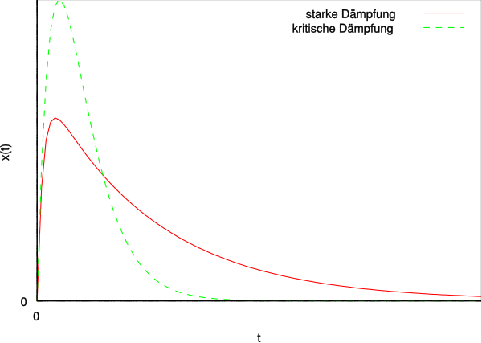
\includegraphics[width=0.45\textwidth]{Versuch_neu_1-2/figures/2285.pdf}
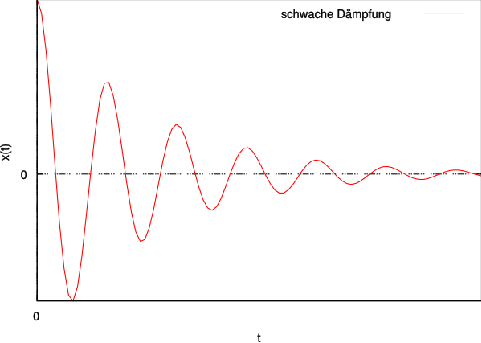
\includegraphics[width=0.45\textwidth]{Versuch_neu_1-2/figures/2284.pdf}
\end{center}
\caption{Zeitlicher Verlauf der Amplitude einer Schwingung im Kriechfall und aperiodischen Grenzfall (links) und im gedämpften Schwingfall (rechts).}
\label{fig:Schwingungen}
\end{figure}

\subsection{Angeregte Schwingung mit Dämpfung}

Wirkt auf das schwingungsfähige System das äußere periodische Anregungsmoment $M\cos(\omega t)$, so wird die Bewegungsgleichung eine inhomogene lineare Differentialgleichung 2. Ordnung. Diese kann man zwar analytisch lösen, was wir hier aber dem ''geneigten Leser'' überlassen wollen.\\
Nach dem Einschwingvorgang, währenddessen die Bewegung des Systems eine Überlagerung der Bewegung mit seiner Eigenfrequenz $\omega_0$ sowie einer mit der Erregerfrequenz $\omega$ ist, lautet die Lösung der Bewegungsgleichung 
\begin{equation}
	\varphi(t) = \frac{N}{\sqrt{\left(\omega_0^2 - \omega^2\right)^2 +4\beta^2\omega^2}}\cos(\omega t - \alpha)\, .
\end{equation}
Dies ist eine Schwingung mit der Frequenz $\omega_e$, welche um den Winkel $\alpha$ gegen die Phase der Erregerschwingung verschoben ist. \\
Wie man sieht, ist die Amplitude 
\begin{equation*}
	\varphi_0 = \frac{N}{\sqrt{\left(\omega_0^2 - \omega^2\right)^2 +4\beta^2\omega^2}}
\end{equation*}
abhängig von der Differenz der Erregerfrequenz zur Eigenfrequenz des Systems $\left(\omega_0^2 - \omega^2\right)^2$ und zur Dämpfung $\beta$. Sie wird maximal, wenn die Erregerfrequenz der \textit{Resonanzfrequenz} entspricht, die sich ergibt als:
\begin{equation}
	\omega_r = \sqrt{\omega_0^2 -2\beta^2}\, .
\end{equation}

\begin{figure}[ht!]
	\centering
	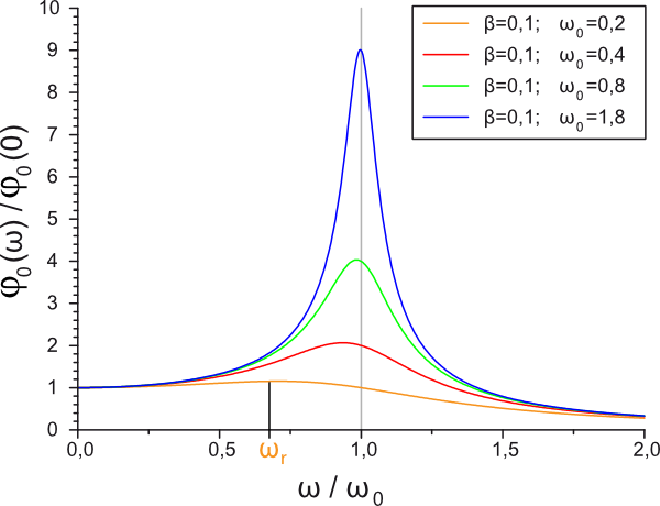
\includegraphics[width=0.45\textwidth]{Versuch_neu_1-2/figures/3946.pdf}
	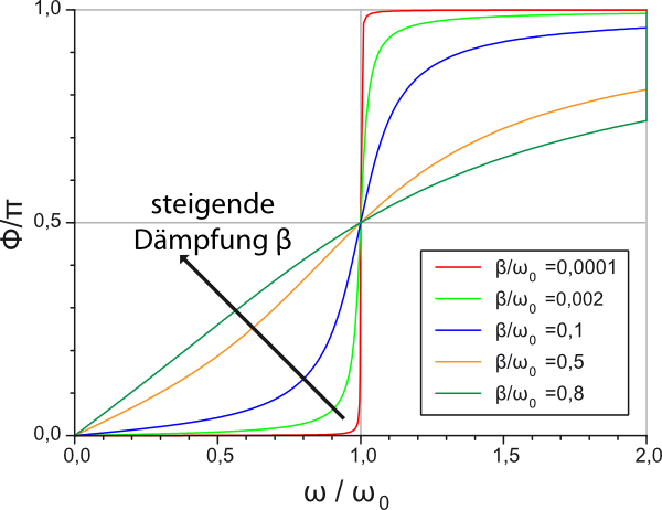
\includegraphics[width=0.45\textwidth]{Versuch_neu_1-2/figures/3947.pdf}
	\caption{Links: Frequenzgang einer angeregten, gedämpften Schwingung für verschiedene Dämpfungen. Beachten Sie die Verschiebung der Resonanzfrequenz. Rechts: Phasenverschiebung einer angeregten, gedämpften Schwingung für verschiedene Dämpfungen.}
	\label{fig:Resonanz}
\end{figure}

Auch die Phasenverschiebung hängt von der Differenz der Erreger- und Eigenfrequenz und der Dämpfung ab:
\begin{equation*}
	\tan\alpha = \frac{2\beta\omega}{\omega_0^2-\omega^2}
\end{equation*}
Wie in Abbildung \ref{fig:Resonanz} zu sehen ist, ist die Phasenverschiebung (für genügend kleine Dämpfung) sehr klein bei Frequenzen kleiner als der Eigenfrequenz des Systems, das System folgt dem Erreger sehr genau. Überschreitet die Erregerfrequenz die Eigenfrequenz, so wird die Phasenverschiebung 90\degree, das System eilt dem Erreger um eine halbe Schwingung hinterher.
%------------------------------------------------
\section{Fragen zur Vorbereitung}
%------------------------------------------------

\begin{enumerate} 
	\item Skizzieren Sie von Hand die Funktion $f(t) = \cos(\omega t)$. Welche Werte nimmt diese an für $\omega t = 0\, , \pi/2\, , \pi\, , 3\pi/4\, , 2\pi$?
	%
	\item Unter welchen Bedingungen tritt eine resonant angeregte Schwingung auf? Wie verhält sich die Amplitude der Schwingung in diesem Fall?
	%
	\item Was ist der konzeptionelle Unterschied zwischen der Frequenz $f$ und der Kreisfrequenz $\omega$?
	%
	\item Wieso ist die detaillierte Kenntnis der Eigenschwingungsfrequenzen von Gebäuden, Brücken oder den Flügeln eines Flugzeuges wichtig?
	%
	\item Beschreiben Sie die Bewegung eines gedämpften, schwingfähigen Systems im Schwingfall, Kriechfall und im aperiodischen Grenzfall? Wann tritt welcher der drei Fälle ein?
\end{enumerate} 

%------------------------------------------------
\section{Durchführung} 
%------------------------------------------------

\subsection{Vorbereitung}

Starten Sie den PC und melden Sie sich als Benutzer »Prakt« (kein Passwort) an. Schalten Sie die Motorsteuerung in dem separaten Kasten auf der Rückseite ein. Starten Sie das Programm »Pohl« über die Verknüpfung auf dem Desktop. Ihre Messdaten werden nach dem Ende jeder einzelnen Messung graphisch dargestellt und sollten umgehend ausgedruckt werden. Zusätzlich wird eine PDF-Datei in dem angegebenen Verzeichnis gespeichert. Bitte nicht in anderen Verzeichnissen Dateien verändern oder löschen.

\subsection{Bedienung des Messprogramms}

Das Programm »Pohl« ist eine grafische Oberfläche für die Messwertaufnahme am Pohlschen Resonator.
\begin{enumerate}
	\item Starten Sie das Programm »Pohl«, falls dies noch nicht geschehen ist.
	%
	\item Legen Sie eine neue Messung an. Geben Sie hierzu die Parameter der Messung in den dafür vorgesehen Textfeldern an, damit diese im Ergebnisgraphen vermerkt werden. Die Frequenz geben Sie bitte in Millihertz (mHz) an, mit der der Exzenter betrieben werden soll. Ein Wert von 250 lässt den Exzenter also in 4 Sekunden eine vollständige Umdrehung durchführen. Bei der Eingabe von 0 ist der Exzenter deaktiviert.
	%
	\item Klicken Sie auf den Button »neue Messung starten«, um eine neue Messreihe anzulegen. Die Datenaufnahme und ggf. auch die Motorsteuerung starten nun.
	%
	\item Das Pohlsche Rad befindet sich nun in Eigenschwingung bzw. im Einschwingvorgang. Dabei wird der Amplitudenverlauf grafisch aufgetragen, sobald das Rad zwecks Kalibrierung der Auslese die Nulllage zwei mal durchlaufen hat (vorher keine Datenanzeige). 
	%
	\item Bei der erzwungenen Schwingung empfiehlt es sich, sobald der Einschwingvorgang beendet ist, die Messung durch einen Klick auf den Button »Messreihe neu starten« erneut zu starten. Bei Messung der Eigenschwingung empfiehlt es sich, gerade bei starker Dämpfung, zunächst die Initialisierung der Elektronik abzuwarten, dann das Rad erneut auszulenken und den Button »Messreihe neu starten« zu betätigen.
	%
	\item Durch einen Klick auf die Reiter »Amplitude« bzw. »Phasenraum« können Sie sich verschiedene Messdaten schon während der Messung anschauen.
	%
	\item Wenn Sie genug Daten haben, beenden Sie die Messung mit einem Klick auf »Messung beenden«. Es wird nachfolgend eine PDF-Datei mit dem graphisch dargestellten Ergebnis angelegt und angezeigt; diese bitte umgehend ausdrucken.
\end{enumerate}

\subsection{Durchführung}

\begin{enumerate}
	% Messung der Eigenfrequenz des Resonators bei Dämpfung 0 --> ablese aus Plot
	\item Bringen Sie den Motor mit dem Messprogramm in Position 0.
	%Messung des Amplitudenverlaufs für verschieden starke Dämpfung --> nur Betrachten?
	\item Starten Sie die Messung für die freie Schwingung für vier verschiedene Stellungen des Millimetertriebs der Wirbelstrombremse: 0, 4, 6 und 8~mm. Die Skala des Millimetertriebs weist dabei ggf. einen Versatz auf: »0 mm« bezieht sich auf die Position bei Deckung der Kante des Magneten mit der Außenseite des Kupferrads und die anderen Angaben gelten relativ dazu. Regen Sie den Resonator bei abgeschaltetem Motor zu Eigenschwingungen an (Anregung 0~Hz; falls nötig die Nulllage des Motors vorher per Software einstellen). Dabei die Auslenkung der Drehscheibe von Hand auf 120° stellen und loslassen. Während einer kurzen Initialisierungsphase der Messelektronik werden noch keine Messdaten angezeigt.
	%
	\item Messen Sie nun bitte die erzwungene gedämpfte Schwingung. Für drei verschiedene Dämpfungen 4, 6 und 8~mm (Stellung am Millimetertrieb der Wirbelstrombremse) führen Sie dazu jeweils die nachfolgenden Schritte durch:
	\begin{enumerate}
		\item Nehmen Sie für die jeweils eingestellte Dämpfung für genügend viele verschiedene Frequenzen (150-600~mHz) die Schwingung des Oszillators auf. Stellen Sie sicher, dass 
		der Einschwingvorgang vorbei ist, bevor Sie die Datenaufzeichnung starten. Hierbei muss die Amplitude des Pohl'schen Resonators zeitlich konstant sein. Achten Sie weiterhin darauf, dass genügend viele Schwingungen aufgezeichnet werden.
		%
		\item Machen Sie insbesondere in der Nähe der Resonanz viele Messungen. Achten Sie dabei jedoch auf eine mögliche Resonanzkatastrophe. In diesem Fall ist die Messung sofort über »Messung beenden« zu beenden.
	\end{enumerate}
\end{enumerate}
Für die Auswertung sind die ausgedruckten Graphen ausreichend. Wer es vorzieht, die PDF-Dateien zu verwenden, sollte diese über das Internet oder einen mitgebrachten USB-Stick übertragen. Am einfachsten geht dies mit einer E-Mail an sich selbst. Ihr/e Betreuer/in kann Ihnen dabei helfen.

%------------------------------------------------
\section{Auswertung} 
%------------------------------------------------

\begin{enumerate}
	%
	\item \label{aw:Schwingfall} Lesen Sie aus den zeitlichen Verläufen der vier verschieden gedämpften Schwingungen deren jeweilige Frequenz $\hat{\omega}$ ab.
	%
	\item \label{aw:Log_Dekrement}Tragen Sie für die vier verschieden gedämpften Schwingungen den Logarithmus der maximalen Auslenkung, $\ln\varphi(t)$ s. Gl. \ref{eq:Amplitude_gedaempft}, als Funktion der Zeit auf. Diesen finden Sie für die Halbwelle mit positiver Auslenkung auf der zweiten Seite des zur Messung gehörenden pdf-Dokumentes. \\
	Lesen Sie aus dem Graphen die Dämpfung $\beta$ inkl. ihrer Unsicherheit ab.
	%
	\item Berechnen Sie mit Hilfe von Gleichung \ref{eq:Schwingfall} für jede der vier verschieden gedämpften Schwingungen jeweils $\omega_0$. Mitteln Sie über diese vier Werte, um die Eigenfrequenz des ungedämpften Systems inklusive ihrer Unsicherheit zu berechnen.
	%
	\item Bestimmen Sie die Amplitude der angeregten Schwingungen für die verschiedenen Erregerfrequenzen aus den zugehörigen Graphen. Mitteln Sie graphisch über mehrere Perioden, indem Sie jeweils eine Gerade parallel zur x-Achse  an die maximalen Amplituden der positiven Halbwellen anpassen. 
	%
	\item Tragen Sie nun das Verhältnis der Amplitude bei der jeweiligen Erregerfrequenz zur Amplitude bei einer Frequenz nahe Null, $\varphi(\omega)/\varphi(0)$, als Funktion des Verhältnisses der Erregerfrequenz zur Eigenfrequenz des ungedämpften Systems, $\omega/\omega_0$, auf. Dabei sollen die Kurven für die verschiedenen Dämpfungen in denselben Graphen eingetragen werden.
\end{enumerate}